\section{Reducing the Model to One Half}

\Citeauthor{akyuz2022} pointed out in their master thesis, that the model satisfies the property in \Cref{equ:yunus.property.symmetry}.
This means, that there is some symmetry in the model.
In the following, I will reduce the model to only $\theta \mapsto F(\theta) \mod \pi$ and observe what happens in the ``type A'' and ``type B'' parameter regions, explored above.
\begin{align}
    F(\theta + \pi) & \equiv F(\theta) + \pi \mod 2 \pi \label{equ:yunus.property.symmetry}
\end{align}

Now, something interesting happens.
\Cref{fig:yunus.pi.2d.full} shows a 2D-scan of the same area that is depicted in \Cref{fig:yunus.2pi.2d.full}.
You can see that the ``type B'' parameter regions now have a different color from the ``type A'' parameter regions.
This means that the cycles in that area now have a higher period.

\begin{figure}
    \centering
    \includegraphics[width=0.6\textwidth]{98_Yunus_modpi/2D_Period_Zoomed/result.png}
    \caption{2D Scan of Halved Original Model}
    \label{fig:yunus.pi.2d.full}
\end{figure}

To understand what is happening, we now look at the cobwebs in this reduced model at the same points we did previously for the full model.
\Cref{fig:yunus.pi.CobwebA6} shows the cycle at point $A$.
It now has period 6 and symbolic sequence $\L^3\R^3$.
So the cycle from the full model was just condensed into two branches.
Similarly, the cycle at point $C$, shown in \Cref{fig:yunus.pi.CobwebC6}, also has period 6 and symbolic sequence $\L^2\R^4$.

The same thing does not work for the stable cycles in the period regions of ``type B''.
Because the cycles there behave differently on each half of the function of the original model.
Instead, the cycles here keep the same period.
And they merge into one stable cycle with the symbolic sequence $\L^3\R^3\L^2\R^4$.
This is similar to the adding of cycles in period adding structures, but here the adding stops after this once.
\todo{citation for period adding}
You can see this when examining the cycle in \Cref{fig:yunus.pi.CobwebB6} closely.
Also, there is only one stable cycle in this parameter region now.
Because the rotation by $\pi$ now is equivalent to the identity.

The meaning of this is secondary.
What is more important, is the practical aspect of detecting ``type B'' parameter regions next to ``type A'' parameter regions in period scans.
We will use this in the future by doing scans of both the full model and the ``halved'' model in interesting regions and comparing these two.

%The reason we have coexistence in the full model and something different in this reduced model is that the cycle in the full model starts on either the first or the second rotation of $\L^3\R^3\L^2\R^4$ in the first half of the full model.
%In the second half, it will have to behave like the other rotation.
%For example, if the cycle starts on $\L^3\R^3$, in the full model this will translate to $\A^3\B^3$.
%Then the cycle will have to behave like the second rotation in the right half of the model.
%The second rotation is $\L^2\R^4$ which translates to $\C^2\D^4$ in the full model.
%Concatenating both halves of the cycle in the full model will yield $\A^3\B^3\C^2\D^4$.
%Analogous, starting on the second rotation $\L^2\R^4$ will yield the second cycle in the full model $\A^2\B^4\C^3\D^3$.

\begin{figure}
    \centering
    \begin{subfigure}{0.3\textwidth}
        \centering
        \includegraphics[width=\textwidth]{98_Yunus_modpi/Period6/Cobweb_A_6/result.png}
        \caption{At Point $A$}
        \label{fig:yunus.pi.CobwebA6}
    \end{subfigure}
    \begin{subfigure}{0.3\textwidth}
        \centering
        \includegraphics[width=\textwidth]{98_Yunus_modpi/Period6/Cobweb_B_6/result.png}
        \caption{At Point $B$}
        \label{fig:yunus.pi.CobwebB6}
    \end{subfigure}
    \begin{subfigure}{0.3\textwidth}
        \centering
        \includegraphics[width=\textwidth]{98_Yunus_modpi/Period6/Cobweb_C_6/result.png}
        \caption{At Point $C$}
        \label{fig:yunus.pi.CobwebC6}
    \end{subfigure}
    \caption{Cobwebs of Halfed Original Model}
\end{figure}
